\documentclass[12pt]{report}

% Paquetes LaTeX y estilos globales
\input{etc/pkgs}
\input{etc/style}

%%%%%%%%%%%%%%%%%%%%%%%%%%%%%%%%%%%%%%%%%%%%%%%%%%%%%%%%%%%%%%%%%%%%%%%%%%%%%%%%%%%%%

% Variables para la portada
\setTitle{Sistema Inteligente de Gestión Logística con ArangoDB}
\setAuthor{Ismael Carrasco Mkhazni \\ Guillermo García León} % Si hay más de un autor, separarlos con \\
\setDegree{Grado en Ingeniería Informática - Ingeniería del Software} % Cambiar si es necesario

%%%%%%%%%%%%%%%%%%%%%%%%%%%%%%%%%%%%%%%%%%%%%%%%%%%%%%%%%%%%%%%%%%%%%%%%%%%%%%%%%%%%%

% Dedicatoria del trabajo
% Si no se desea incluir, comentar o borrar la línea siguiente para eliminar la página de dedicatoria

%%%%%%%%%%%%%%%%%%%%%%%%%%%%%%%%%%%%%%%%%%%%%%%%%%%%%%%%%%%%%%%%%%%%%%%%%%%%%%%%%%%%%

% Comienzo del documento
\begin{document}

    % Portada y secciones no numeradas
    \input{sections/00_portada}
    \chapter*{Resumen}
Este proyecto presenta el diseño e implementación de una plataforma de gestión logística avanzada utilizando una base de datos multimodelo (ArangoDB). El sistema permite gestionar una red de almacenes y productos mediante grafos, optimizando el cálculo de rutas y el control de inventarios en tiempo real. La solución se despliega mediante una arquitectura contenedorizada con Docker y una interfaz reactiva en Streamlit.
\vspace{.5cm}

\textbf{Palabras clave:} ArangoDB, Grafos, Logística, AQL, Docker, Streamlit.
    \chapter*{Abstract}
This project presents the design and implementation of an advanced logistics management platform using a multi-model database (ArangoDB). The system allows managing a network of warehouses and products using graphs, optimizing route calculation and real-time inventory control. The solution is deployed using a containerized architecture with Docker and a reactive interface in Streamlit.

\vspace{.5cm}

\textbf{Keywords:} ArangoDB, Graphs, Logistics, AQL, Docker, Streamlit.
    
    % Índice del documento y de figuras
    \begingroup
        % Los enlaces son normalmente azules, pero en los índices se configuran a negro para que no aparezca todo azul
        \hypersetup{linkcolor=black}
        \tableofcontents
        \listoffigures
        \listoftables
        \lstlistoflistings
    \endgroup
    
    % Cambia el estilo de números de página de romanos a normal
    \clearpage\pagenumbering{arabic}
    
    % Capítulos del trabajo
    %\input{sections/ejemplos_borrame}
    \chapter{Introducción}\label{cap:introduccion}

El propósito de este trabajo es resolver la complejidad inherente a la logística de distribución mediante el uso de bases de datos de grafos. En lugar de utilizar modelos relacionales tradicionales que sufren con consultas recursivas pesadas al intentar modelar redes, he optado por ArangoDB para modelar almacenes como nodos y rutas como aristas, permitiendo una adaptabilidad inmediata ante cambios en el entorno.

La metodología seguida ha sido iterativa: partiendo de un diseño de esquema básico, progresé hasta lograr una arquitectura modular robusta, enfrentándome a retos técnicos tanto en la lógica de resolución de rutas óptimas mediante AQL como en la orquestación del despliegue en contenedores Docker, los cuales se detallan en los posteriores capítulos de implementación.
    \chapter{Estudio previo}\label{cap:planificación}

\section{Introducción}
Breve introducción al capítulo

\section{ArangoDB}
Es una base de datos NoSQL nativa multimodelo, lo que significa que permite trabajar con documentos, grafos y sistemas clave-valor utilizando un único motor central y un mismo lenguaje de consultas llamado AQL (ArangoDB Query Language).

\section{Arquitectura Multimodelo}
En el mundo de las bases de datos, normalmente estás atado a un solo formato: tablas (relacional), documentos tipo JSON (como MongoDB), o grafos (como Neo4j).

La principal ventaja de la arquitectura multimodelo nativa de ArangoDB es que combina varios modelos en un mismo motor central, permitiendo acceder a ellos con el mismo lenguaje de consultas (AQL). Los tres modelos que soporta son:
\begin{itemize}
\item \textbf{Documentos:} Para guardar información jerárquica y flexible.
\item \textbf{Grafos:} Para definir relaciones complejas y direcciones entre los datos.
\item \textbf{Clave-Valor:} Para accesos de lectura ultrarrápidos mediante un identificador único.
\end{itemize}

\section{Modelado de Grafos y AQL}
En una base de datos tradicional, buscar conexiones requiere cruzar tablas mediante operaciones costosas. En un modelo de grafos, las relaciones son importantes y trazarlas es directo e inmediato.
AQL (ArangoDB Query Language) es el lenguaje que permite recorrer esta red de datos. .

\section{Integración}

    \chapter{Análisis del problema}\label{cap:analisis}

\section{Introducción}
En este capítulo detallamos los requisitos fundamentales que el sistema logístico debe satisfacer. El análisis se ha abordado desde una perspectiva integral, considerando tanto la robustez necesaria en la persistencia y el cálculo de datos en el backend  como la agilidad requerida en la interfaz de usuario para una gestión operativa real.

\section{Requisitos de información}
Para modelar fielmente la red logística, el sistema debe ser capaz de persistir y relacionar entidades que poseen atributos tanto técnicos como descriptivos para su visualización:

\begin{itemize}
    \item \textbf{Almacenes (Nodos):} Además de su identificación y capacidad, deben incluir metadatos de localización (como ciudad o coordenadas) que permitan su representación en el mapa interactivo.
    \item \textbf{Productos (Nodos):} Deben categorizarse mediante identificadores únicos (SKU), nombres descriptivos y categorías para facilitar su filtrado en el inventario.
    \item \textbf{Conexiones Viales (Aristas):} Deben definir la topología de la red, vinculando almacenes mediante el atributo de distancia, esencial para los algoritmos de optimización.
    \item \textbf{Existencias (Aristas):} Representan la relación dinámica entre productos y almacenes, manteniendo un conteo preciso de unidades disponibles en cada punto de la red.
\end{itemize}

\section{Requisitos funcionales}
Hemos definido las capacidades del sistema centrándonos en la utilidad para el administrador final, equilibrando la potencia de cálculo con la facilidad de uso:

\begin{itemize}
    \item \textbf{Gestión de Red Interactiva:} El sistema debe permitir realizar operaciones CRUD sobre almacenes, productos y rutas. Estas acciones deben reflejarse inmediatamente tanto en la base de datos como en la representación visual de la red.
    \item \textbf{Cálculo de Rutas Críticas:} Implementar una lógica capaz de determinar el camino más corto entre dos puntos, garantizando que el algoritmo recorra exclusivamente las rutas de transporte válidas.
    \item \textbf{Dashboard de Inventario:} Proporcionar una visión clara del stock vivo, permitiendo realizar ajustes de unidades y visualizar la distribución de productos a través de la red.
    \item \textbf{Visualización Dinámica de la Red:} La interfaz debe generar un grafo interactivo que ayude al usuario a comprender la topología de la red logística de un solo vistazo.
    \item \textbf{Resiliencia ante Contingencias:} Capacidad de recalcular rutas de forma automática si una conexión queda inhabilitada, asegurando la continuidad de la cadena de suministro.
\end{itemize}

\section{Requisitos no funcionales}
Para asegurar la calidad técnica y la facilidad de evaluación del proyecto, hemos establecido los siguientes criterios:
\begin{itemize}
    \item \textbf{Portabilidad:} El sistema debe ser agnóstico al entorno de ejecución, garantizando su funcionamiento inmediato mediante el uso de contenedores.
    \item \textbf{Rendimiento en Relaciones:} La arquitectura debe permitir realizar consultas de vecindad y caminos cortos sin la penalización de rendimiento propia de los sistemas relacionales convencionales.
    \item \textbf{Persistencia y Consistencia:} Se debe asegurar que las operaciones sobre el grafo mantengan la integridad de la red, evitando nodos o aristas huérfanas tras una eliminación.
\end{itemize}

    \chapter{Diseño de la solución}\label{cap:diseño}

\section{Introducción}
La base de datos se ha estructurado como un grafo multimodelo denominado \texttt{RedLogistica}. A diferencia de las bases de datos relacionales estándar, este modelo me permite recorrer conexiones logísticas con una eficiencia de orden de complejidad mucho menor.

\section{Modelo de Datos y Diagrama}
La organización lógica de las colecciones diseñadas en ArangoDB es la siguiente:
\begin{itemize}
    \item \textbf{Vértices (Documentos):} \texttt{Almacenes} y \texttt{Productos}.
    \item \textbf{Aristas (Edges):} \texttt{Rutas} (conecta almacenes entre sí, incluyendo el atributo \texttt{distancia\_km}) y \texttt{Stock\_en} (conecta productos con almacenes, incluyendo el atributo de \texttt{cantidad}).
\end{itemize}

En la Figura \ref{fig:grafo_db} se ilustra la topología de la base de datos mediante un diagrama conceptual.

\begin{figure}[htp]
    \centering
    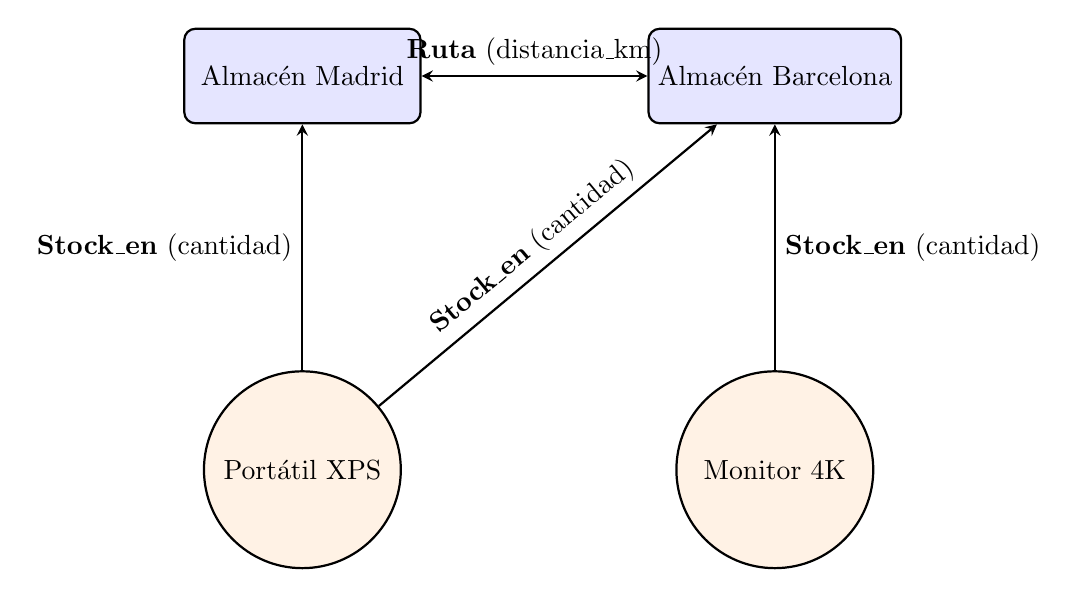
\begin{tikzpicture}[node distance=4cm, auto, thick, >=stealth]
        % Definición de estilos
        \tikzstyle{nodoAlmacen} = [draw, rectangle, rounded corners, fill=blue!10, minimum width=3cm, minimum height=1.2cm, text centered]
        \tikzstyle{nodoProducto} = [draw, circle, fill=orange!10, minimum size=2.5cm, text centered]

        % Nodos Almacenes
        \node[nodoAlmacen] (almacenMadrid) {Almacén Madrid};
        \node[nodoAlmacen, right of=almacenMadrid, xshift=2cm] (almacenBarna) {Almacén Barcelona};
        
        % Nodos Productos
        \node[nodoProducto, below of=almacenMadrid, yshift=-1cm] (prodPortatil) {Portátil XPS};
        \node[nodoProducto, below of=almacenBarna, yshift=-1cm] (prodMonitor) {Monitor 4K};

        % Aristas
        \draw[<->] (almacenMadrid) -- node[above] {\textbf{Ruta} (distancia\_km)} (almacenBarna);
        \draw[->] (prodPortatil) -- node[left] {\textbf{Stock\_en} (cantidad)} (almacenMadrid);
        \draw[->] (prodMonitor) -- node[right] {\textbf{Stock\_en} (cantidad)} (almacenBarna);
        \draw[->] (prodPortatil) -- node[above, sloped] {\textbf{Stock\_en} (cantidad)} (almacenBarna);
    \end{tikzpicture}
    \caption{Diagrama topológico del grafo \texttt{RedLogistica} y sus relaciones.}
    \label{fig:grafo_db}
\end{figure}

\section{Decisiones de Diseño: Integridad en Grafos}
Una decisión arquitectónica crítica a la que tuve que enfrentarme fue la gestión de la integridad referencial. Dado que ArangoDB no impone restricciones rígidas de borrado en cascada de la misma forma que un motor SQL, tuve que implementar lógica AQL manual transaccional. Esto garantiza que, si se elimina un almacén del sistema por necesidades de negocio, se supriman simultáneamente todas sus rutas adyacentes y registros de stock vinculados, previniendo la existencia de "aristas huérfanas" que pudieran corromper consultas futuras.

\section{Conclusiones}
El diseño propuesto explota las ventajas de los grafos nativos para resolver un problema de red complejo, garantizando al mismo tiempo la consistencia de los datos mediante una capa lógica de control implementada directamente en el código de backend.
    \chapter{Implementación}\label{cap:implementacion}

\section{Introducción}
Este capítulo describe el proceso de construcción real del sistema, detallando el stack tecnológico seleccionado y las soluciones de ingeniería aplicadas para organizar el código y sortear los problemas de despliegue.

\section{Herramientas y Tecnologías}
\begin{itemize}
    \item \textbf{Base de Datos:} ArangoDB configurado para persistencia de grafos multimodelo.
    \item \textbf{Backend:} Python 3.10 utilizando el controlador oficial \texttt{python-arango}.
    \item \textbf{Frontend:} Streamlit, empleado para desarrollar una interfaz reactiva.
    \item \textbf{Despliegue:} Orquestación de servicios mediante \texttt{docker-compose}, aislando la base de datos (\texttt{db}) de la aplicación (\texttt{app}).
\end{itemize}

\section{Arquitectura: Patrón Repositorio}
A medida que el proyecto crecía, la clase gestora original corría el riesgo de convertirse en un antipatrón \textit{God Class} (una única clase abarcando toda la funcionalidad). Para refactorizarlo, apliqué el Patrón Repositorio dividiendo el sistema en módulos lógicos:
\begin{enumerate}
    \item \texttt{database.py}: Dedicado en exclusiva a la gestión de la conexión y la instanciación.
    \item \texttt{crud.py}: Contiene clases aisladas (\texttt{CRUDAlmacenes}, \texttt{CRUDRutas}, etc.) que abstraen la lógica AQL de cada dominio.
\end{enumerate}

\section{Resolución de Conflictos Técnicos}
Durante la integración de Docker, me enfrenté a un error de importación circular en Python (\texttt{ModuleNotFoundError}) provocado por una colisión de \textit{namespaces} al renombrar el directorio principal de la aplicación. Logré solucionarlo modificando el punto de entrada a \texttt{main.py} y, fundamentalmente, configurando la variable de entorno \texttt{PYTHONPATH=/app} dentro del contenedor, forzando al intérprete a resolver correctamente la jerarquía de directorios.

\section{Conclusiones}
La implementación resultante demuestra ser modular, mantenible y altamente portable gracias al esfuerzo puesto en la correcta contenedorización del entorno de ejecución.
    \chapter{Pruebas}\label{cap:pruebas}

\section{Introducción}
Las pruebas del sistema se han enfocado en validar la exactitud algorítmica en el recorrido de grafos y en comprobar la capacidad dinámica del sistema frente a alteraciones inesperadas en la topología de la red.

\section{Validación del Algoritmo de Rutas}
Durante la evaluación de las consultas AQL, detectamos una anomalía semántica importante: el algoritmo \texttt{SHORTEST\_PATH} nativo tendía a utilizar los nodos de \texttt{Productos} como atajos entre ciudades, dado que estas aristas no contaban con atributo de distancia. Esto devolvía rutas carentes de sentido físico (ej. 350 km entre Madrid y Valencia saltando a través de un producto). 

Logramos resolver este comportamiento restringiendo explícitamente el motor AQL para que evaluara de manera exclusiva la colección de aristas \texttt{Rutas}, obligando al algoritmo de Dijkstra interno a considerar únicamente carreteras reales. Tras aplicar esta restricción, las métricas fueron exactas.

\section{Simulación de Contingencias}
Para verificar la resiliencia del modelo, desarrollamos un test de estrés eliminando deliberadamente la arista principal que conectaba Madrid y Barcelona (simulando un accidente o corte vial). Al volver a solicitar el recálculo de la ruta óptima, el sistema reaccionó con una adaptabilidad inmediata: redirigió el flujo logístico a través de nodos intermedios alternativos (vía Bilbao) y ajustó la distancia total de 620 km a 1010 km de manera totalmente transparente, sin requerir una sola modificación en la lógica de backend.

\section{Conclusiones}
Las pruebas confirman el éxito rotundo del modelo orientado a grafos. El sistema reacciona en tiempo real a los cambios estructurales, demostrando que ArangoDB es una solución técnica superior para la planificación logística.

    \chapter{Conclusiones}\label{cap:conclusiones}

El desarrollo integral de este sistema logístico ha servido para validar de forma empírica la idoneidad de las bases de datos de grafos para la resolución de problemas de enrutamiento que, históricamente, penalizan severamente el rendimiento en sistemas de naturaleza relacional o tabular.

El uso de un diseño multimodelo en ArangoDB ha simplificado drásticamente el modelo mental del dominio de negocio. Paralelamente, la adopción del Patrón Repositorio en la capa de software ha asegurado un código legible y escalable. La contenedorización completa del ciclo de vida del proyecto mediante Docker me ha permitido ofrecer una solución ``llave en mano'', mitigando la clásica problemática de las dependencias locales y garantizando un despliegue transparente para su evaluación.

Aunque la curva de aprendizaje inicial del lenguaje AQL y del razonamiento transversal en grafos fue pronunciada, los resultados técnicos conseguidos demuestran una capacidad resolutiva sólida y justifican plenamente la elección tecnológica, logrando una plataforma altamente tolerante a fallos logísticos.

\section*{Uso de Herramientas de IA}
En cumplimiento con las directrices de la asignatura "Complementos de Bases de Datos", declaramos el uso de modelos generativos de IA (Gemini, de Google) como herramienta de apoyo técnico durante el desarrollo del proyecto. Sus usos específicos han sido:
\begin{itemize}
    \item \textbf{Análisis Arquitectónico y Refactorización:} Soporte consultivo en la transición del código de un modelo centralizado a uno distribuido (Patrón Repositorio) para la separación de responsabilidades en la base de datos.
    \item \textbf{Depuración de Despliegue:} Asistencia técnica puntual en la comprensión de jerarquías de directorios dentro de Docker para resolver el fallo de importación circular (\texttt{PYTHONPATH}).
    \item \textbf{Formato y Estilo:} Apoyo en la adaptación y formateo de la documentación técnica al lenguaje de marcado LaTeX.
\end{itemize}

Como autores de la entrega, declaramos que todo el código fuente y el contenido teórico generado ha sido analizado de manera crítica, depurado y validado empíricamente a través de nuestras pruebas. Comprendoemos en profundidad cada bloque lógico y componente del sistema expuesto en esta memoria.

    % Bibliografía
    \bibliographystyle{unsrtnat}
    \bibliography{bibliografia.bib}
        

% Fin del documento
\end{document}
